% !TeX root = ..\main.tex
\section{Lựa chọn công nghệ}

    \subsection{Front-end}
        \subsubsection{React}
            \hspace*{0.5cm} React là một thư viện JavaScript được phát triển bởi Facebook, là kiểu lập trình khai báo giúp người dùng xây dựng giao diện người dùng (UI) một cách hiệu quả và linh hoạt. React cho phép ta tạo những giao diện (UI) phức tạp từ những "component" mà mỗi component đó chính là một đoạn code nhỏ và độc lập. Khi chia ra từng component giúp ta có thể tái sử dụng lại tốt. Mỗi component có thể có các state bên trong nó và quản lý state đó, ngoài ra các component có thể nhận các dữ liệu từ các component khác truyền vào thông qua các props, và mỗi component sẽ chỉ re-render khi các state hay props của component thay đổi, vậy nên các component sẽ không cần re-render khi không cần thiết.\\
            
            \begin{figure}[!htp]
                \begin{center}
                
\includegraphics[width=5cm]{img/Technology/react.png}
                \end{center}
                \caption{Logo React \cite{technologyReact}}
            \end{figure}

            Ưu điểm của React \cite{technologyReactAdvance}:
            \begin{itemize}
                \item Dễ hiểu và dễ sử dụng: Nguồn cung cấp tài liệu, hướng dẫn và tài nguyên đào tạo tốt giúp ta có thể học và hiểu React một cách dễ dàng. Đặc biệt đối với những ai đã có nền tảng về Javascript thì React khá dễ sử dụng.
                \item Các component có thể tái sử dụng: Mỗi component trong ứng dụng đều có thể tái sử dụng. Là trung tâm của tất cả các ứng dụng khi sử dụng React, các component có thể được lồng vào nhau. Việc lồng component này với component khác cho phép tạo ra các giao diện phức tạp được xây dựng từ các khối component đơn giản.
                \item Nâng cao hiệu suất: React là tạo nên một hiệu suất tuyệt vời vì nó sử dụng cách quản lý một DOM ảo. DOM xử lý HTML, XML hoặc XHTML. Nó là một API lập trình và đa nền tảng. Với React, người dùng không viết trực tiếp vào DOM mà vào DOM ảo, do đó dẫn đến hiệu suất mượt mà và nhanh hơn.
                \item Có thư viện JavaScript: React cung cấp một thư viện JavaScript rất phong phú, do đó mang lại sự linh hoạt hơn cho các lập trình viên.
            \end{itemize}

            Nhược điểm của React \cite{technologyReactAdvance}:
            \begin{itemize}
                \item Cần cập nhật liên tục: Tốc độ phát triển cao của React dẫn đến môi trường thay đổi nhanh chóng và liên tục, điều này làm cho lập trình viên khó có thể áp dụng tất cả. Do đó, lập trình viên cần phải luôn cập nhật những thay đổi về kỹ năng hay môi trường.
                \item Quản lý component: Khi số lượng component trong hệ thống đạt tới một số lượng lớn nhất định, việc quản lý và chọn lựa component phù hợp trở nên tốn thời gian hơn đòi hỏi cách tổ chức và quản lý component phải hợp lý. Khi không tổ chức các component một cách có hệ thống thì khiến cho việc quyết định tìm kiếm để sử dụng lại component gặp khó khăn và xảy ra việc viết một component mới bị trùng với một component đã có nhưng không tìm thấy, khiến tăng số lượng component cũng như chi phí về lưu trữ code.
                \item Quản lý state: Trong các component luôn phải thực hiện quản lý các state, các component lồng nhau thì compoent con có thể nhận state của component cha qua props, mà khi lồng ghép quá nhiều component khiến cho việc truyền state từ component này sang component kia trở nên quá cồng kềnh.
            \end{itemize}
        \subsubsection{Ant Design Pro}
            \hspace*{0.5cm} Ant Design Pro là một front-end framework bao gồm 2 thành phần chính được sử dụng để hỗ trợ xây dựng giao diện trong đề tài này là Ant Design và DvaJs.
            \subsubsubsection{Ant Design}
            \hspace*{0.5cm} Ant Design là một thư viện của React cung cấp rất nhiều component có tính thông dụng cao, đa dạng và đầy đủ để đáp ứng các nhu cầu để không cần phải định nghĩa thêm các base component nữa. Ant Design có một cộng đồng sử dụng rất lớn, hiện tại số lượt started ở trên github của Ant Design đã đạt hơn 83 nghìn lượt \cite{technologyAntdStar}.
            
            \begin{figure}[!htp]
                \begin{center}
                
\includegraphics[width=5cm]{img/Technology/antd.jpg}
                \end{center}
                \caption{Logo Ant Design \cite{technologyAntd}}
            \end{figure}

            \hspace*{0.5cm} Ưu điểm của Ant Design bao gồm:
            \begin{itemize}
                \item Số lượng base component: Như đã giới thiệu, Ant Design cung cấp rất nhiều base component đa dạng và đầy đủ giúp ta không cần sài thêm thư viện giao diện khác nữa.
                \item Khả năng customize base component: Ant Design cung cấp rất nhiều props để lập trình viên có thể tùy biến linh hoạt theo nhu cầu.
                \item Dễ học, dễ hiêu: Ant Design cung cấp bộ tài liệu hướng dẫn rất chi tiết cùng với demo tương ứng giúp người dùng có thể dễ dàng hiểu rõ và sử dụng.
                \item Responsive: Ant Design hỗ trợ dàn layout tương thích trên nhiều thiết bị và loại màn hình khác nhau, vì vậy không cần phải sài thêm các thư viện khác để responsive.
                \item Cộng đồng sử dụng: Ant Design có cộng đồng sử dụng lớn giúp cho việc tìm kiếm giải đáp thắc mắc rất dễ dàng.
            \end{itemize}

            \subsubsubsection{DvaJs}
            \hspace*{0.5cm} Dva là một giải pháp luồng dữ liệu dựa trên redux và redux-saga. Để đơn giản hóa trải nghiệm của việc phát triển, dva cũng tích hợp cả react-router và fetch. Có thể xem dva là một khung ứng dụng của React để đơn giản hóa API và giúp việc phát triển các ứng dụng React trở nên thuận tiện và nhanh hơn.\\

            \begin{figure}[!htp]
                \begin{center}
                
\includegraphics[width=5cm]{img/Technology/dva.png}
                \end{center}
                \caption{Logo DvaJs \cite{technologyDva}}
            \end{figure}

            Dva xử lý các vấn đề về việc giao tiếp giữa các component trong React khi các component cần sử dụng chung state trở nên quá cồng kềnh bằng cách tập trung các state lại 1 nơi, đồng thời giúp quản lý những side effect (những thứ liên quan đến bất đồng bộ) trong ứng dụng dễ dàng hơn đồng thời kiểm tra và xử lý lỗi tốt hơn.\\

            \begin{figure}[!htp]
                \begin{center}
                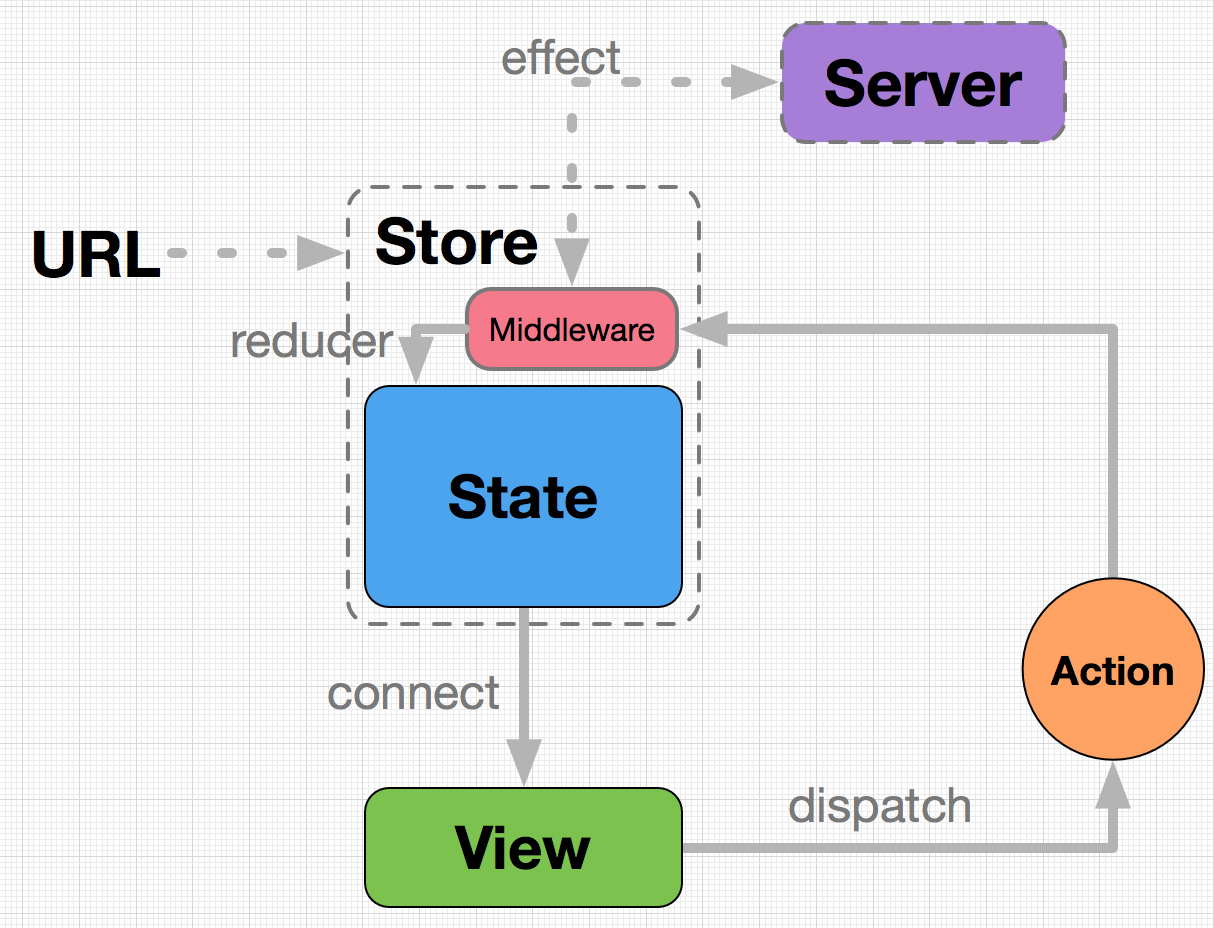
\includegraphics[width=10cm]{img/Technology/dva-struct.png}
                \end{center}
                \caption{Mô hình data flow trong dva \cite{technologyDvaAdvance}}
            \end{figure}

            Các thành phần chính trong dva bao gồm \cite{technologyDvaAdvance}: 
            \begin{itemize}
                \item \textbf{State:} đây là một đối tượng chứa toàn bộ trạng thái ứng dụng. State là nơi lưu trữ dữ liệu, và dữ liệu sẽ được cập nhật sau khi nhận được Action.
                \item \textbf{Action:} là một đối tượng được sử dụng để mô tả các sự kiện của lớp giao diện người dùng.
                \item \textbf{Reducer:} là một bộ xử lý Action, được sử dụng để xử lý các hoạt động đồng bộ. Chức năng của Reducer là xử lý state hiện tại từ state trước đó tương ứng theo Action được gửi đến để xử lý.
                \item \textbf{Effect:} cũng là một bộ xử lý Action, được sử dụng để xử lý các hoạt động bất đồng bộ. Thường dùng cho các hoạt động I/O hay đọc ghi cơ sở dữ liệu.
                \item \textbf{View:} là lớp giao diện người dùng bao gồm các thành phần React. Sau khi tìm nạp dữ liệu từ State, nó sẽ hiển thị dữ liệu đó thành mã HTML. Chỉ cần State thay đổi thì View sẽ được cập nhật tự động.
            \end{itemize}

            % \hspace*{0.5cm} Ở phần front-end, nhóm sử dụng bộ 
    
    \subsection{Back-end}
\par Ở phần back-end, nhóm sử dụng ngôn ngữ Golang để hiện thực. Đây là một ngôn ngữ mới và hiệu quả cho việc xây dựng hệ thống nói chung, và xây dựng hệ thống microservice nói riêng.
Những lợi ích mà Golang có bao gồm:
\begin{itemize}
    \item Golang là ngôn ngữ static-typed, kiểu dữ liệu của biến là cố định và được khai báo từ đầu. Do đó các lỗi xảy ra liên quan đến kiểu dữ liệu đều được phát hiện và ngăn chặn ở bước compile. Ngoài ra tính năng thu gom rác (Garbage collection) giúp Golang quản lý bộ nhớ an toàn và hạn chế lỗi xuất hiện.
    \item Golang là ngôn ngữ đơn giản và dễ học. Cú pháp đơn giản và trực quan của Golang giúp cho ngôn ngữ này được ưa thích và người dùng có thể học dễ dàng.
    \item Golang là ngôn ngữ phổ biến, được sử dụng rộng rãi. Ngôn ngữ này được tạo nên và phát triển bởi Google, cùng cộng đồng lớn, do đó việc học và tìm sự trợ giúp khi sử dụng Golang trở nên dễ dàng hơn.
    \item Thời gian build và thực thi thấp hơn. Golang được tối ưu để thời gian build và chạy ít hơn.
    \item Golang hỗ trợ mạnh việc lập trình concurrency. Điều này giúp các ứng dụng Golang có khả năng mở rộng lớn.
\end{itemize}
\par Qua đó, có thể thấy Golang có nhiều ưu điểm khi sử dụng. Với lợi thế về hiệu năng, khả năng mở rộng và độ tin cậy, Golang là lựa chọn thích hợp cho nhóm trong dự án này.